\documentclass[12pt]{article}
\usepackage[margin=1in]{geometry}
\usepackage{tikz}
\usetikzlibrary{arrows.meta}
\usepackage{times}
\usepackage{parskip}
\usepackage{graphicx}

\begin{document}

% ========== Title Page ==========
\begin{center}
\vspace*{2cm}
{\LARGE \textbf{Literature Survey}}\\[0.8cm]
{\Large for ButterFlight}\\[3cm]
{\large By: Cecilia Chen and Yiding Tian}\\[5cm]
{\large CIS 6600}\\[0.2cm]
{\large Advanced Topics in Computer Graphics and Animation}\\[0.5cm]
{\large Instructor: Dr.~Stephen Lane}
\end{center}

\newpage

% ========== Introduction ==========
\section*{Introduction}

Realistic modeling and simulation of living things has found numerous applications in
entertainment, virtual worlds, education, and behavioral analysis. In recent years,
various efforts have been attempted to model and animate a variety of flying creatures,
including birds [WP03][Ju13], dragonflies, bats, and insects [WJDZ14][WRJM15].
However, realistically simulating butterfly flights for real-time graphics and animation
applications remains an under-explored problem. Experiment-based methods have
difficulty acquiring full trajectories of real-world butterflies; CFD-based methods are
computationally too expensive for real-time simulation; and, unlike many flying insects,
a butterfly flies with small flapping frequencies and exhibits closely coupled
wing-body interaction that cannot be ignored.

Our authoring tool, ButterFlight, is based on the practical force-based model
proposed by Chen et al.\ [CLTL22]. This approach first models a butterfly with
parametric maneuvering functions including wing-abdomen interaction, then simulates
dynamic maneuvering control through a force model that includes both a simplified
aerodynamics force and a curl-noise vortex force.

In this literature survey, we trace three converging research threads that lead to
[CLTL22]: (1)~from the seminal quasi-steady aerodynamic theory for insect flight
[Ell84], through bird and butterfly flight animation, to the parametric maneuvering
functions for butterfly wing-body motion; (2)~from the seminal Boids flocking model
[Rey87], through biologically-plausible insect swarm simulation, to the chaotic
trajectory generation for flying insects; and (3)~from Perlin noise [Per02] and
curl-noise [BHN07], to the vortex force model that drives inherent noisy behavior
in butterfly flight.


% ========== Content ==========
\newpage
\section*{Content}

The research evolution is shown in the following graph:

\begin{figure}[ht]
\centering
\resizebox{\textwidth}{!}{%
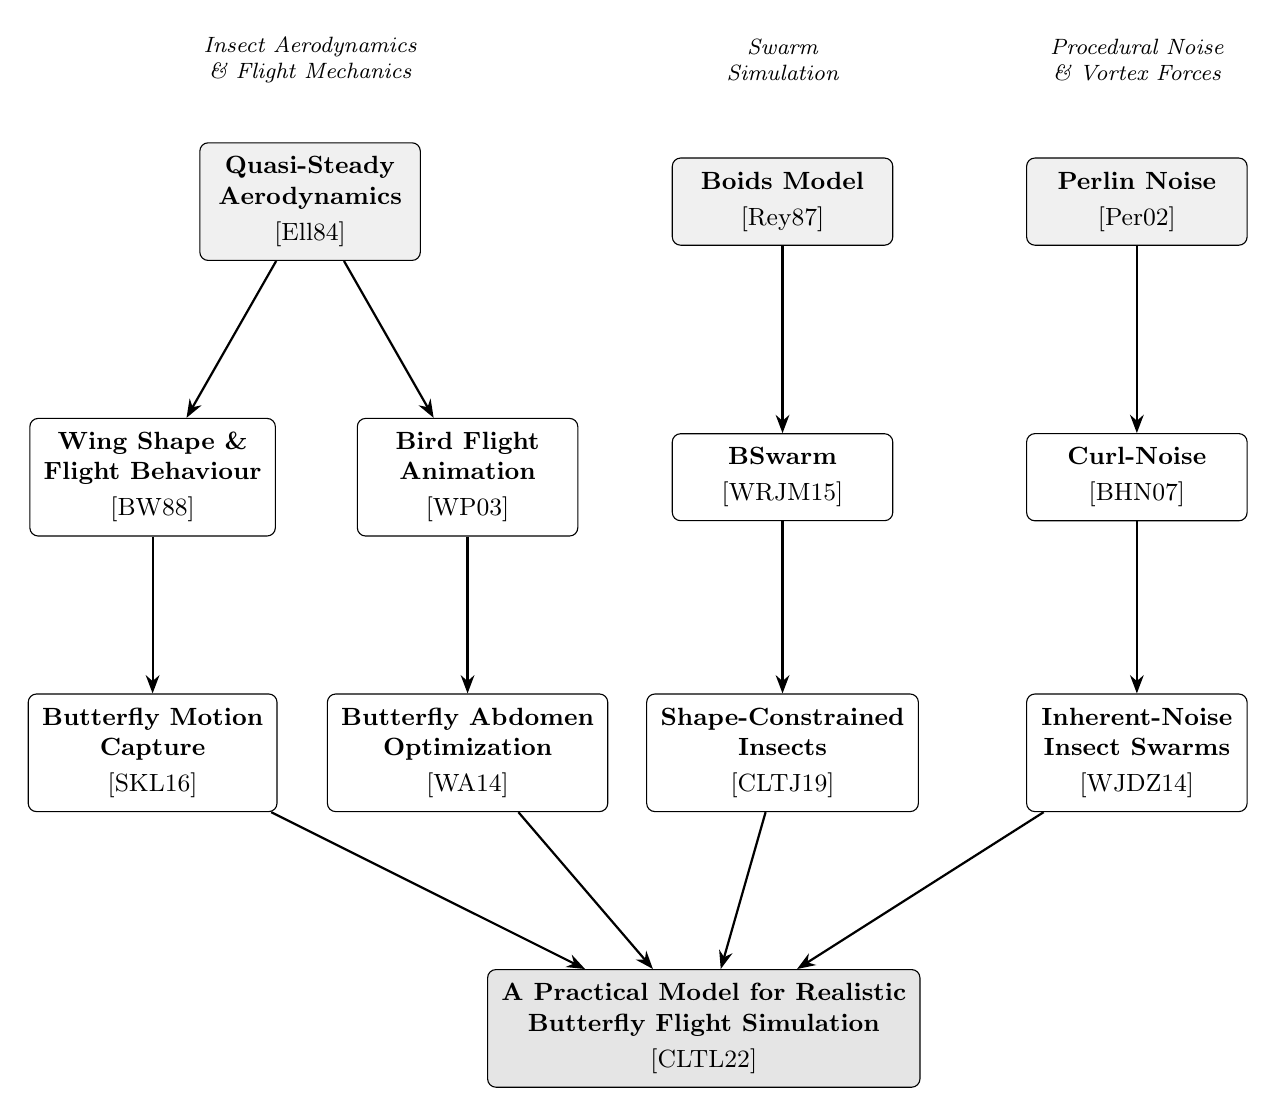
\begin{tikzpicture}[
  box/.style={draw, rectangle, rounded corners=3pt, align=center,
              inner sep=5pt, minimum width=2.8cm, font=\small},
  seminal/.style={box, fill=gray!12},
  target/.style={box, fill=gray!20, minimum width=5cm},
  branch/.style={font=\footnotesize\itshape, align=center},
  >=Stealth
]

% ---- Branch labels ----
\node[branch] at (-5, 1.8) {Insect Aerodynamics\\\& Flight Mechanics};
\node[branch] at (1, 1.8) {Swarm\\Simulation};
\node[branch] at (5.5, 1.8) {Procedural Noise\\\& Vortex Forces};

% ---- Row 0: Seminal works ----
\node[seminal] (ell) at (-5, 0) {
  \textbf{Quasi-Steady}\\
  \textbf{Aerodynamics}\\[2pt]
  {[Ell84]}
};
\node[seminal] (rey) at (1, 0) {
  \textbf{Boids Model}\\[2pt]
  {[Rey87]}
};
\node[seminal] (per) at (5.5, 0) {
  \textbf{Perlin Noise}\\[2pt]
  {[Per02]}
};

% ---- Row 1 ----
\node[box] (bw) at (-7, -3.5) {
  \textbf{Wing Shape \&}\\
  \textbf{Flight Behaviour}\\[2pt]
  {[BW88]}
};
\node[box] (wp) at (-3, -3.5) {
  \textbf{Bird Flight}\\
  \textbf{Animation}\\[2pt]
  {[WP03]}
};
\node[box] (wrjm) at (1, -3.5) {
  \textbf{BSwarm}\\[2pt]
  {[WRJM15]}
};
\node[box] (bhn) at (5.5, -3.5) {
  \textbf{Curl-Noise}\\[2pt]
  {[BHN07]}
};

% ---- Row 2 ----
\node[box] (skl) at (-7, -7) {
  \textbf{Butterfly Motion}\\
  \textbf{Capture}\\[2pt]
  {[SKL16]}
};
\node[box] (wa) at (-3, -7) {
  \textbf{Butterfly Abdomen}\\
  \textbf{Optimization}\\[2pt]
  {[WA14]}
};
\node[box] (cltj) at (1, -7) {
  \textbf{Shape-Constrained}\\
  \textbf{Insects}\\[2pt]
  {[CLTJ19]}
};
\node[box] (wjdz) at (5.5, -7) {
  \textbf{Inherent-Noise}\\
  \textbf{Insect Swarms}\\[2pt]
  {[WJDZ14]}
};

% ---- Row 3: Our paper ----
\node[target] (cltl) at (0, -10.5) {
  \textbf{A Practical Model for Realistic}\\
  \textbf{Butterfly Flight Simulation}\\[2pt]
  {[CLTL22]}
};

% ---- Edges ----
\draw[->, thick] (ell) -- (bw);
\draw[->, thick] (ell) -- (wp);
\draw[->, thick] (rey) -- (wrjm);
\draw[->, thick] (per) -- (bhn);

\draw[->, thick] (bw) -- (skl);
\draw[->, thick] (wp) -- (wa);
\draw[->, thick] (wrjm) -- (cltj);
\draw[->, thick] (bhn) -- (wjdz);

\draw[->, thick] (skl) -- (cltl);
\draw[->, thick] (wa) -- (cltl);
\draw[->, thick] (cltj) -- (cltl);
\draw[->, thick] (wjdz) -- (cltl);

\end{tikzpicture}%
}
\caption{Research Evolution Graph}
\end{figure}


% ========== Paper Descriptions ==========

\bigskip\noindent
\textbf{[Ell84]} In this seminal work, Ellington establishes the quasi-steady
aerodynamic theory for analyzing hovering insect flight. The framework computes
instantaneous lift and drag forces on insect wings based on the angle of attack,
wing area, and air velocity, using empirically derived lift and drag coefficients.
This quasi-steady analysis became the standard approach for modeling the
aerodynamic forces of flapping insect wings without resorting to computationally
expensive CFD solvers. In Chen et al.\ [CLTL22], the simplified aerodynamic force
equations (Equations~4--6) are built directly on this theory.

\bigskip\noindent
\textbf{[Rey87]} Reynolds introduced the Boids model, a seminal distributed
behavioral model for simulating flocks, herds, and schools. Each agent follows
three simple local rules---separation, alignment, and cohesion---to produce
emergent collective behavior. This work laid the foundation for all subsequent
swarm simulation methods. However, the basic Boids model does not support
physical forces for realistic simulation. Later works extended these ideas with biologically-motivated
spatial zones (repulsion, alignment, attraction), which in turn led to the insect
swarm models that feed into [CLTL22].

\bigskip\noindent
\textbf{[Per02]} Perlin improved his original noise function with better gradient
computation and reduced directional artifacts. This procedural noise generation
technique became fundamental to many graphics applications, from terrain generation
to texture synthesis. In the context of butterfly simulation, Perlin noise is
integrated into the curl-noise vortex force (Equation~7 in [CLTL22]) to produce
the time-varying, spatially coherent noise field that drives the inherent chaotic
behavior of butterfly flight.

\bigskip\noindent
\textbf{[BW88]} Betts and Wootton present the first detailed kinematic
investigation of butterflies performing varied patterns of natural flight. Six
butterfly species flying freely in the field were filmed with a high-speed cin\'e
camera and subjected to kinematic and morphometric analysis. They characterized
flight modes---fast forward, slow forward, hovering, and climbing---and found
correlations between flight performance and wing shape parameters including
aspect ratio, wing loading, and moments of wing inertia. Their finding that
butterflies exhibit great flight versatility through startling shifts in frequency,
amplitude, and stroke plane angle motivates the parametric maneuvering approach
used in [CLTL22].

\bigskip\noindent
\textbf{[WP03]} Wu and Popovi\'c apply aerodynamic theory to animate realistic
bird wing flapping. They introduce parametric maneuvering functions to control
wing motion during flight and optimize the maneuvering parameters of both wings
and feathers through an offline method. This was the first work to bridge
aerodynamic force models with computer graphics animation of flapping flight. The
periodic maneuvering function design used in Chen et al.\ [CLTL22] (Equation~1)
is directly inspired by this work and by [WA14].

\bigskip\noindent
\textbf{[BHN07]} Bridson, Houriham, and Nordenstam propose curl-noise as a
procedural approach for generating divergence-free velocity fields for fluid flow
simulation. By taking the curl of a potential field constructed from Perlin noise,
the method produces incompressible, collision-free flow fields. Chen et al.\
[CLTL22] extends this approach to compute an artificial vortex force acting on
the butterfly thorax (Equation~7), simulating the wake influence of wing flapping
and the inherent noisy behavior observed in real butterflies.

\bigskip\noindent
\textbf{[WRJM15]} Wang et al.\ propose BSwarm, a biologically-plausible dynamics
model for insect swarms. This work, from the same research group (co-authors Jin and Manocha) as
[CLTL22], established the framework for biologically-grounded insect swarm
animation. However, BSwarm and similar swarm methods focus on macro-level swarm
trajectories, using pre-created cycle-frames for individual insect motion---a
limitation that [CLTL22] addresses with its micro-level force-based model.

\bigskip\noindent
\textbf{[WJDZ14]} Wang et al.\ apply a curl-noise field to compute
collision-free trajectories for flying insects, capturing the inherent noisy
dynamics of insect swarms. This was the first work to combine procedural
curl-noise with swarm simulation for flying insects, establishing the use of
curl-noise in insect animation. From the same research group (co-authors Jin and
Deng) as [CLTL22], this work focused on macro-level swarm trajectories.
Chen et al.\ [CLTL22] extends the curl-noise idea from macro-level swarm
trajectories to micro-level individual butterfly motion via the vortex force
applied to the thorax.

\bigskip\noindent
\textbf{[SKL16]} Sridhar, Kang, and Landrum use 12 high-resolution VICON
motion-tracking cameras to capture the free flight of Monarch butterflies. They
quantify body orientation---thorax and abdomen separately---and wing kinematics as
a six-degree-of-freedom system, along with instantaneous lift coefficient during
climbing flight. Critically, they show that the wing flapping frequency and body
oscillation frequency match at approximately 9.5~Hz, confirming the close coupling
between wing and body motion. They also provide key morphological data (wing area,
body mass) that are used as simulation parameters in [CLTL22] (Table~2). The
finding that the abdomen rotates with opposite phase to wing flapping directly
informs the phase angle settings in Equation~1 of [CLTL22].

\bigskip\noindent
\textbf{[WA14]} Wilson and Albertani optimize wing-flapping and abdomen actuation
parameters for hovering in the butterfly \textit{Idea leuconoe}. They model the
butterfly as a rigid body while integrating the abdomen's inertia and moment, and
design periodic functions for the coupled wing and abdomen motion. Along with
[WP03], this work directly inspires the periodic maneuvering function design in
Chen et al.\ [CLTL22] (Equation~1). A related work by Sridhar, Kang, and Lee
(2020) further develops a geometric formulation for Monarch butterfly dynamics
with abdomen undulation effects, confirming that the abdomen moves with opposite
phase to wing flapping during hovering and climbing.

\bigskip\noindent
\textbf{[CLTJ19]} Chen et al.\ extend the
chaotic behavior of flying insects to generate special-effect animations with
shape constraints. Building on the swarm simulation foundation of [WRJM15] and
[WJDZ14], this work demonstrates artistically controllable insect swarm motion.
It serves as a direct predecessor to [CLTL22], which shifts focus from macro-level
swarm effects to a physically-grounded, micro-level individual butterfly flight
model with wing-body interaction.

\bigskip\noindent
\textbf{[CLTL22]} Chen et al.\ propose a first-of-its-kind, practical model to
simulate realistic butterfly flights. The approach consists of three
inter-connected modules: (1)~butterfly modeling with a hierarchical skeleton and
parametric maneuvering functions including wing-abdomen interaction, inspired by
[WP03] and [WA14]; (2)~forces computation combining simplified aerodynamic forces
based on quasi-steady theory [Ell84] with a curl-noise vortex force [BHN07] for
inherent noisy behavior; and (3)~maneuvering control through body motion
decoupling that generates both inherently noisy trajectories and rapidly-adjusted
body postures. The approach is validated through simulations of various scenarios
(path following, wind interaction, chasing, aggregation, traveling) and user
studies, demonstrating real-time performance at 60~FPS for single butterflies
and 25~FPS for swarms of 100.

\newpage

% ========== References ==========
\section*{References}

\noindent
[BHN07] BRIDSON R., HOURIHAM J., NORDENSTAM M.: Curl-noise for
procedural fluid flow. \textit{ACM Transactions on Graphics (TOG)} 26, 3
(2007), 46--es.

\medskip\noindent
[BW88] BETTS C.~R., WOOTTON R.~J.: Wing shape and flight behaviour in
butterflies (Lepidoptera: Papilionoidea and Hesperioidea): a preliminary
analysis. \textit{Journal of Experimental Biology} 138, 1 (1988), 271--288.

\medskip\noindent
[CLTJ19] CHEN Q., LUO G., TONG Y., JIN X., DENG Z.: Shape-constrained
flying insects animation. \textit{Computer Animation and Virtual Worlds} 30,
3--4 (2019), e1902.

\medskip\noindent
[CLTL22] CHEN Q., LU T., TONG Y., LUO G., JIN X., DENG Z.: A Practical
Model for Realistic Butterfly Flight Simulation. \textit{ACM Transactions on
Graphics (TOG)} 1, 1 (2022), 12 pages.

\medskip\noindent
[Ell84] ELLINGTON C.~P.: The aerodynamics of hovering insect flight. I.
The quasi-steady analysis. \textit{Philosophical Transactions of the Royal
Society of London. B, Biological Sciences} 305, 1122 (1984), 1--15.

\medskip\noindent
[Per02] PERLIN K.: Improving noise. In \textit{ACM Transactions on Graphics
(TOG)}, Vol.~21. ACM, 2002, pp.~681--682.

\medskip\noindent
[Rey87] REYNOLDS C.~W.: Flocks, herds and schools: A distributed behavioral
model. In \textit{Proceedings of the 14th Annual Conference on Computer
Graphics and Interactive Techniques} (1987), pp.~25--34.

\medskip\noindent
[SKL16] SRIDHAR M., KANG C.-K., LANDRUM D.~B.: Instantaneous lift and
motion characteristics of butterflies in free flight. In \textit{46th AIAA
Fluid Dynamics Conference} (2016), 3252.

\medskip\noindent
[WA14] WILSON T., ALBERTANI R.: Wing-flapping and abdomen actuation
optimization for hovering in the butterfly \textit{Idea leuconoe}. In
\textit{52nd Aerospace Sciences Meeting} (2014), 0009.

\medskip\noindent
[WJDZ14] WANG X., JIN X., DENG Z., ZHOU L.: Inherent noise-aware insect
swarm simulation. In \textit{Computer Graphics Forum}, Vol.~33. Wiley Online
Library, 2014, pp.~51--62.

\medskip\noindent
[WP03] WU J., POPOVI\'C Z.: Realistic modeling of bird flight animations.
\textit{ACM Transactions on Graphics (TOG)} 22, 3 (2003), 888--895.

\medskip\noindent
[WRJM15] WANG X., REN J., JIN X., MANOCHA D.: BSwarm:
biologically-plausible dynamics model of insect swarms.
\textit{Proceedings of the 14th ACM SIGGRAPH/Eurographics Symposium on
Computer Animation} (2015), 111--118.

\end{document}
